\documentclass[tikz, border=20pt]{standalone}
\usetikzlibrary{positioning, shapes.gates.logic.US, calc}


\begin{document}

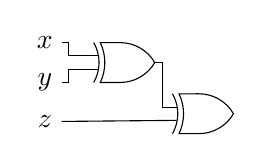
\begin{tikzpicture}

    %Inputs
    \node (x) at (0,0) {$x$};
    \node (y) at (0,-0.5) {$y$};
    \node (z) at (0,-1) {$z$};

    %Gates
    \node[xor gate US, draw] (xor) at ($(x)+(1.0, -0.25)$) {};
    \node[xor gate US, draw] (xor2) at ($(z)+(2.0, 0.10)$) {};

    
    %Lines
    \draw (x) -- ($(x)+(0.3, 0)$) |-  (xor.input 1);
    \draw (y) -- ($(y)+(0.3, 0)$) |-  (xor.input 2);
    \draw (xor.output) -- ($(xor) + (0.5, 0.0)$) |- (xor2.input 1);
    \draw (z) -- (xor2.input 2);
\end{tikzpicture}




\end{document}
